\element{ecart}{
\begin{question}{ecart 01}
Soit le schéma-bloc suivant. On donne $C(p)=1$ et $H(p) = \dfrac{K}{1+\tau p}$.
\begin{center}
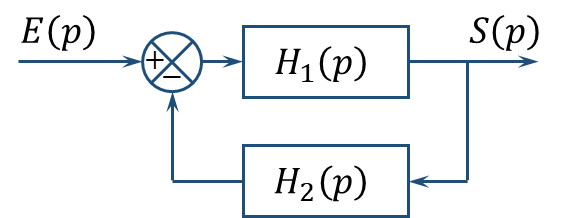
\includegraphics[width=8cm]{fig_01}
\end{center}
	Donner l'écart statique pour un échelon d'amplitude $E_0$.
	\begin{reponses}	
	\bonne{$\varepsilon_s = \dfrac{E_0}{1+K}$}
	\mauvaise {$\varepsilon_s = 0$}
	\mauvaise {$\varepsilon_s = \infty$}
	\mauvaise{$\varepsilon_s = \dfrac{1}{1+K}$}
	\mauvaise{$\varepsilon_s = \dfrac{E_0}{K}$}
	\mauvaise{$\varepsilon_s = \dfrac{1}{K}$}
	\mauvaise{Je ne sais pas calculer simplement.}
	\end{reponses}

\end{question}\\}

\element{ecart}{
\begin{question}{ecart 02}
Soit le schéma-bloc suivant. On donne $C(p)=1$ et $H(p) = \dfrac{K}{1+\tau p}$.
\begin{center}
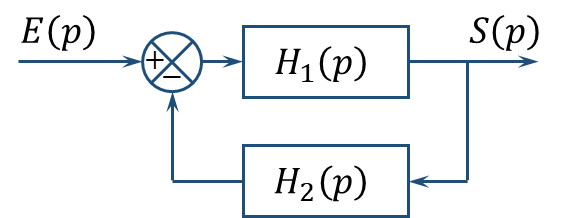
\includegraphics[width=8cm]{fig_01}
\end{center}
	Donner l'écart de trainage pour une rampe de pente $k$.
	\begin{reponses}	
	\bonne      {$\varepsilon_t = \infty$}
	\mauvaise {$\varepsilon_t = \dfrac{k}{1+K}$}
	\mauvaise {$\varepsilon_t = 0$}
	\mauvaise {$\varepsilon_t = \dfrac{1}{1+K}$}
	\mauvaise {$\varepsilon_t = \dfrac{k}{K}$}
	\mauvaise {$\varepsilon_t = \dfrac{1}{K}$}
	\mauvaise{Je ne sais pas calculer simplement.}
	\end{reponses}
\end{question}\\}

\element{ecart}{
\begin{question}{ecart 03}
Soit le schéma-bloc suivant. On donne $C(p)=K_p \left(1+\dfrac{1}{Tp}\right)$ et $H(p) = \dfrac{K}{1+\tau p}$.
\begin{center}
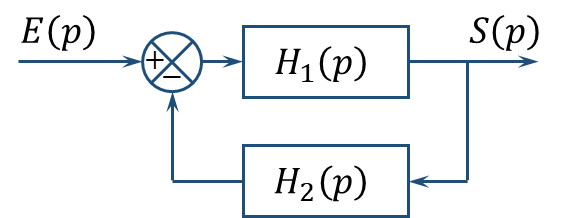
\includegraphics[width=8cm]{fig_01}
\end{center}
	Donner l'écart statique pour un échelon d'amplitude $E_0$.
	\begin{reponses}	
	\bonne{$\varepsilon_s = 0$}
	\mauvaise {$\varepsilon_s = \dfrac{E_0}{1+K}$}
            \mauvaise {$\varepsilon_s = \dfrac{E_0}{1+KK_P}$}
	\mauvaise {$\varepsilon_s = \infty$}
	\mauvaise{$\varepsilon_s = \dfrac{1}{1+KK_P/T}$}
	\mauvaise{$\varepsilon_s = \dfrac{E_0}{K}$}
	\mauvaise{$\varepsilon_s = \dfrac{1}{K}$}
	\mauvaise{Je ne sais pas calculer simplement.}
	\end{reponses}
\end{question}\\}



\element{ecart}{
\begin{question}{ecart 04}
Soit le schéma-bloc suivant. On donne $C(p)=K_p \left(1+\dfrac{1}{Tp}\right)$ et $H(p) = \dfrac{K}{1+\tau p}$.
\begin{center}
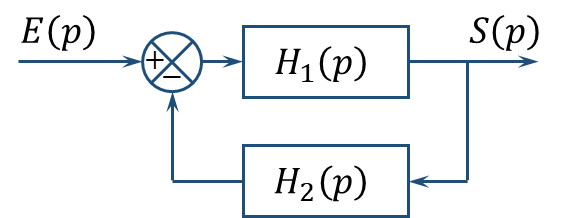
\includegraphics[width=8cm]{fig_01}
\end{center}
	Donner l'écart de trainage pour une rampe de pente $k$.
	\begin{reponses}
	\bonne{$\varepsilon_t = \dfrac{kT}{K_P K}$}
	\mauvaise {$\varepsilon_t = \dfrac{k}{K_P}$}
	\mauvaise {$\varepsilon_t = \dfrac{k}{K_P K}$}
	\mauvaise {$\varepsilon_t = 0$}
           \mauvaise {$\varepsilon_t = \dfrac{T}{K_P K}$}
	\mauvaise{$\varepsilon_t = \dfrac{1}{1+K}$}
	\mauvaise{$\varepsilon_t = \dfrac{k}{1+K}$}
	\mauvaise{$\varepsilon_t = \dfrac{k}{K}$}
	\mauvaise{Je ne sais pas calculer simplement.}
	\end{reponses}
\end{question}\\}

\element{ecart}{
\begin{question}{ecart 05}
Soit le schéma-bloc suivant. On donne $C(p)=1$ et $H(p) = \dfrac{K}{1+\tau p}$.
\begin{center}
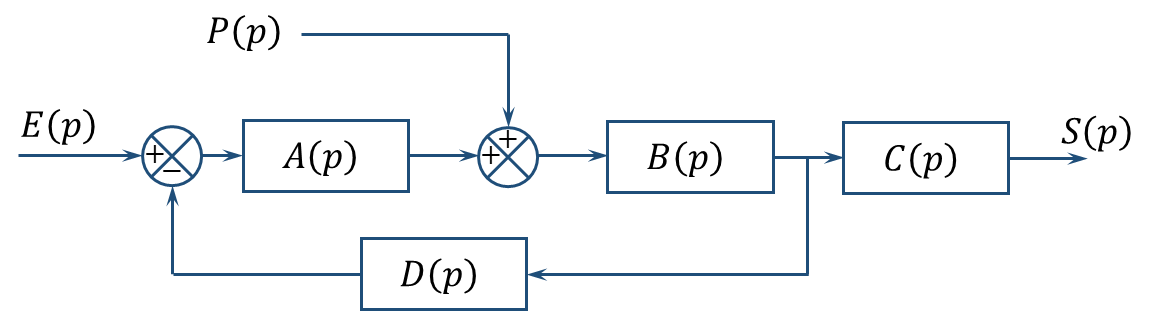
\includegraphics[width=8cm]{fig_02}
\end{center}
	Donner l'écart statique pour un échelon d'amplitude $E_0$. La perturbation sera un échelon d'amplitude $P_0$.
	\begin{reponses}	
	\mauvaise {$\varepsilon_s = \dfrac{E_0}{1+K}+\dfrac{P_0}{1+K}$}
	\mauvaise {$\varepsilon_s = 0$}
	\mauvaise {$\varepsilon_s = \infty$}
	\mauvaise{$\varepsilon_s = \dfrac{E_0}{1+K}$}
	\mauvaise{$\varepsilon_s = \dfrac{P_0}{1+K}$}
	\mauvaise{$\varepsilon_s = \dfrac{1}{K}$}
	\bonne{Je ne sais pas calculer simplement.}
	\end{reponses}

\end{question}\\}

\element{ecart}{
\begin{question}{ecart 06}
Soit le schéma-bloc suivant. On donne $C(p)=1$ et $H(p) = \dfrac{K}{1+\tau p}$.
\begin{center}
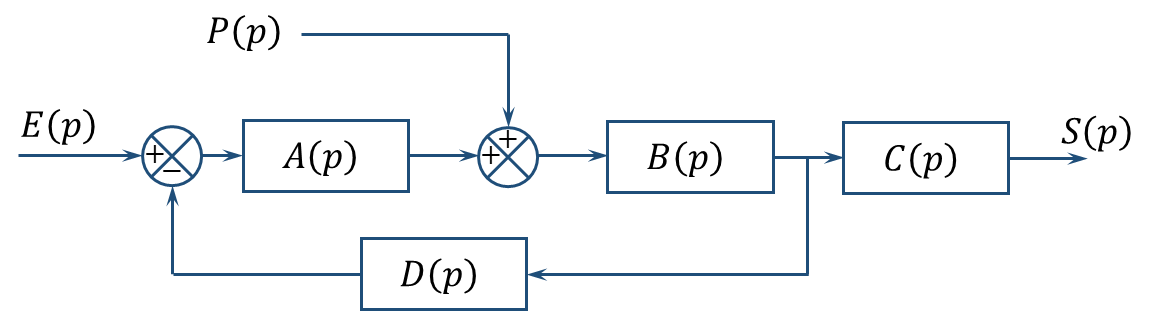
\includegraphics[width=8cm]{fig_02}
\end{center}
	Donner l'écart de trainage pour une rampe de pente $k$. La perturbation sera un échelon d'amplitude $P_0$.
	\begin{reponses}	
	\mauvaise {$\varepsilon_t = \infty$}
	\mauvaise {$\varepsilon_t = \dfrac{k}{1+K}$}
	\mauvaise {$\varepsilon_t = 0$}
	\mauvaise {$\varepsilon_t = \dfrac{1}{1+K}$}
	\mauvaise {$\varepsilon_t = \dfrac{E_0}{1+K} + \dfrac{k}{1+K}$}
	\mauvaise {$\varepsilon_t = \dfrac{1}{K}$}
	\bonne {Je ne sais pas calculer simplement.}
	\end{reponses}
\end{question}\\}

\element{ecart}{
\begin{question}{ecart 07}
Soit le schéma-bloc suivant. On donne $C(p)=K_p \left(1+\dfrac{1}{Tp}\right)$ et $H(p) = \dfrac{K}{1+\tau p}$.
\begin{center}
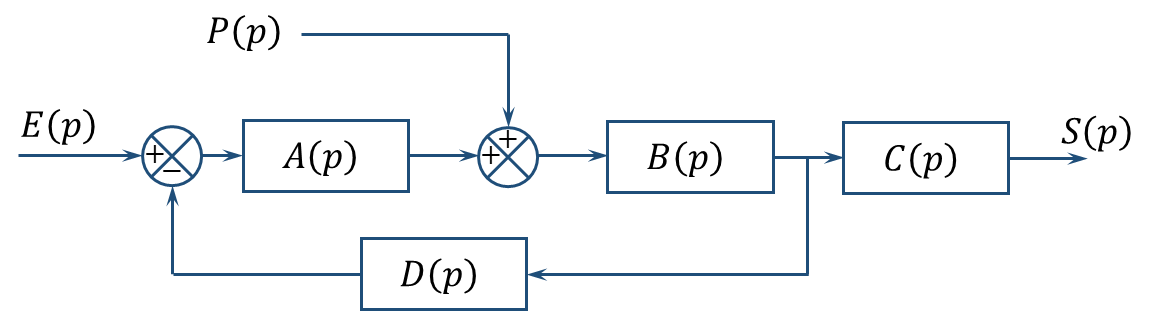
\includegraphics[width=8cm]{fig_02}
\end{center}
	Donner l'écart statique pour un échelon d'amplitude $E_0$. La perturbation sera un échelon d'amplitude $P_0$.
	\begin{reponses}	
	\bonne{$\varepsilon_s = 0$}
	\mauvaise {$\varepsilon_s = \dfrac{E_0}{1+K}$}
            \mauvaise {$\varepsilon_s = \dfrac{E_0}{1+KK_P}$}
	\mauvaise {$\varepsilon_s = \infty$}
	\mauvaise{$\varepsilon_s = \dfrac{1}{1+KK_P/T}$}
	\mauvaise{$\varepsilon_s = \dfrac{E_0}{K}$}
	\mauvaise{$\varepsilon_s = \dfrac{1}{K}$}
	\mauvaise{Je ne sais pas calculer simplement.}
	\end{reponses}
\end{question}\\}



\element{ecart}{
\begin{question}{ecart 8}
Soit le schéma-bloc suivant. On donne $C(p)=K_p \left(1+\dfrac{1}{Tp}\right)$ et $H(p) = \dfrac{K}{1+\tau p}$.
\begin{center}
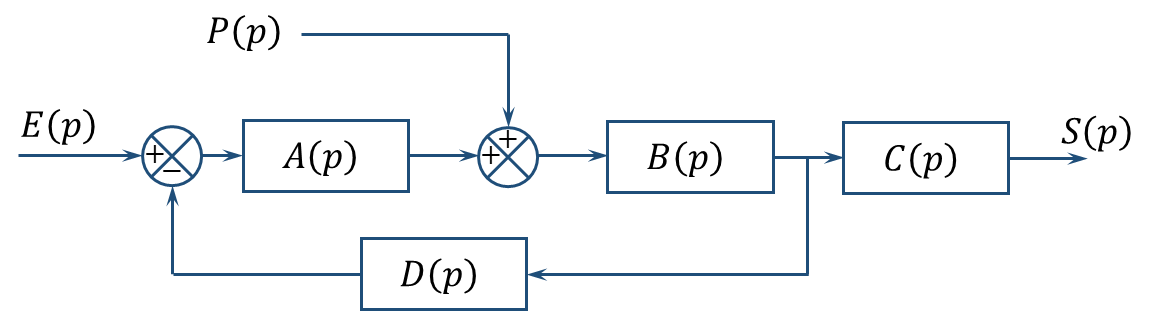
\includegraphics[width=8cm]{fig_02}
\end{center}
	Donner l'écart de trainage pour une rampe de pente $k$. La perturbation sera un échelon d'amplitude $P_0$.
	\begin{reponses}
	\bonne{Je ne sais pas calculer simplement.}
	\mauvaise {$\varepsilon_t = 0$}
	\mauvaise {$\varepsilon_t = +\infty$}
	\mauvaise {$\varepsilon_t = \dfrac{kT}{K_P K}+\dfrac{P_0T}{K_P K}$}
	\mauvaise {$\varepsilon_t = \dfrac{kT}{K_P K}$}
	\mauvaise {$\varepsilon_t = \dfrac{P_0T}{K_P K}$}
	\end{reponses}
\end{question}\\}


\element{ecart}{
\begin{question}{ecart 09}
Soit le schéma-bloc suivant. On donne $C(p)=1$ et $H(p) = \dfrac{K}{p\left(1+\tau p\right)}$.
\begin{center}
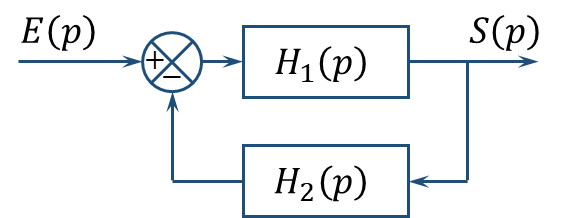
\includegraphics[width=8cm]{fig_01}
\end{center}
	Donner l'écart statique pour un échelon d'amplitude $E_0$.
	\begin{reponses}	
	\mauvaise {$\varepsilon_s = \dfrac{E_0}{1+K}$}
	\bonne{$\varepsilon_s = 0$}
	\mauvaise {$\varepsilon_s = \infty$}
	\mauvaise{$\varepsilon_s = \dfrac{1}{1+K}$}
	\mauvaise{$\varepsilon_s = \dfrac{E_0}{K}$}
	\mauvaise{$\varepsilon_s = \dfrac{1}{K}$}
	\mauvaise{Je ne sais pas calculer simplement.}
	\end{reponses}

\end{question}\\}

\element{ecart}{
\begin{question}{ecart 10}
Soit le schéma-bloc suivant. On donne $C(p)=1$ et $H(p) = \dfrac{K}{p\left(1+\tau p\right)}$.
\begin{center}
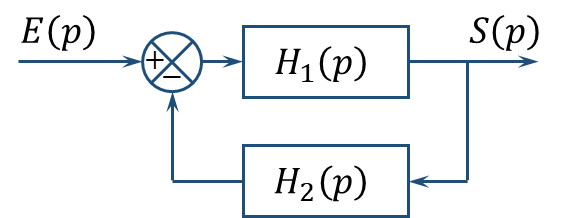
\includegraphics[width=8cm]{fig_01}
\end{center}
	Donner l'écart de trainage pour une rampe de pente $k$.
	\begin{reponses}	
	\mauvaise  {$\varepsilon_t = \infty$}
	\mauvaise {$\varepsilon_t = \dfrac{k}{1+K}$}
	\mauvaise {$\varepsilon_t = 0$}
	\mauvaise {$\varepsilon_t = \dfrac{1}{1+K}$}
	\bonne {$\varepsilon_t = \dfrac{k}{K}$}
	\mauvaise {$\varepsilon_t = \dfrac{1}{K}$}
	\mauvaise{Je ne sais pas calculer simplement.}
	\end{reponses}
\end{question}\\}

\element{ecart}{
\begin{question}{ecart 11}
Soit le schéma-bloc suivant. On donne $C(p)=K_p \left(1+\dfrac{1}{Tp}\right)$ et $H(p) = \dfrac{K}{p\left(1+\tau p\right)}$.
\begin{center}
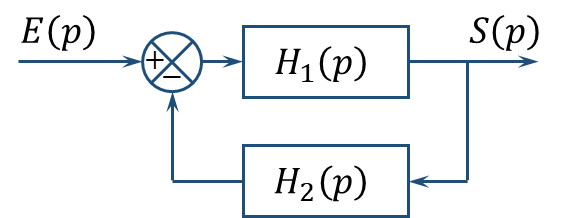
\includegraphics[width=8cm]{fig_01}
\end{center}
	Donner l'écart statique pour un échelon d'amplitude $E_0$.
	\begin{reponses}	
	\bonne{$\varepsilon_s = 0$}
	\mauvaise {$\varepsilon_s = \dfrac{E_0}{1+K}$}
            \mauvaise {$\varepsilon_s = \dfrac{E_0}{1+KK_P}$}
	\mauvaise {$\varepsilon_s = \infty$}
	\mauvaise{$\varepsilon_s = \dfrac{1}{1+KK_P/T}$}
	\mauvaise{$\varepsilon_s = \dfrac{E_0}{K}$}
	\mauvaise{$\varepsilon_s = \dfrac{1}{K}$}
	\mauvaise{Je ne sais pas calculer simplement.}
	\end{reponses}
\end{question}\\}



\element{ecart}{
\begin{question}{ecart 12}
Soit le schéma-bloc suivant. On donne $C(p)=K_p \left(1+\dfrac{1}{Tp}\right)$ et $H(p) = \dfrac{K}{p\left(1+\tau p\right)}$.
\begin{center}
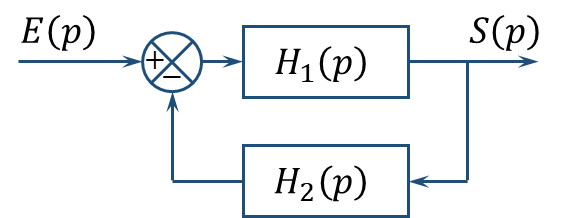
\includegraphics[width=8cm]{fig_01}
\end{center}
	Donner l'écart de trainage pour une rampe de pente $k$.
	\begin{reponses}
	\mauvaise      {$\varepsilon_t = \dfrac{kT}{K_P K}$}
	\mauvaise {$\varepsilon_t = \dfrac{k}{K_P}$}
	\mauvaise {$\varepsilon_t = \dfrac{k}{K_P K}$}
	\bonne {$\varepsilon_t = 0$}
           \mauvaise {$\varepsilon_t = \dfrac{T}{K_P K}$}
	\mauvaise{$\varepsilon_t = \dfrac{1}{1+K}$}
	\mauvaise{$\varepsilon_t = \dfrac{k}{1+K}$}
	\mauvaise{$\varepsilon_t = \dfrac{k}{K}$}
	\mauvaise{Je ne sais pas calculer simplement.}
	\end{reponses}
\end{question}\\}

\element{ecart}{
\begin{question}{ecart 13}
Soit le schéma-bloc suivant. On donne $C(p)=1$ et $H(p) = \dfrac{K}{p\left(1+\tau p\right)}$.
\begin{center}
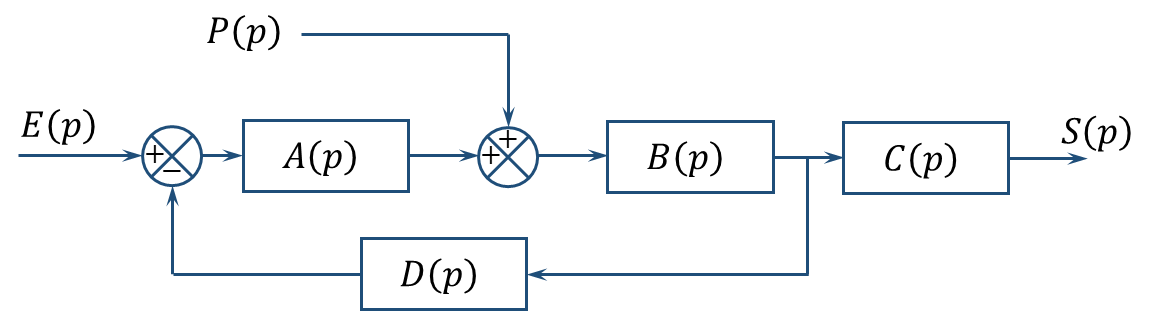
\includegraphics[width=8cm]{fig_02}
\end{center}
	Donner l'écart statique pour un échelon d'amplitude $E_0$. La perturbation sera un échelon d'amplitude $P_0$.
	\begin{reponses}	
	\mauvaise {$\varepsilon_s = \dfrac{E_0}{1+K}+\dfrac{P_0}{1+K}$}
	\mauvaise {$\varepsilon_s = 0$}
	\mauvaise {$\varepsilon_s = \infty$}
	\mauvaise{$\varepsilon_s = \dfrac{E_0}{1+K}$}
	\mauvaise{$\varepsilon_s = \dfrac{P_0}{1+K}$}
	\mauvaise{$\varepsilon_s = \dfrac{1}{K}$}
	\bonne{Je ne sais pas calculer simplement.}
	\end{reponses}

\end{question}\\}

\element{ecart}{
\begin{question}{ecart 14}
Soit le schéma-bloc suivant. On donne $C(p)=1$ et $H(p) = \dfrac{K}{p\left(1+\tau p\right)}$.
\begin{center}
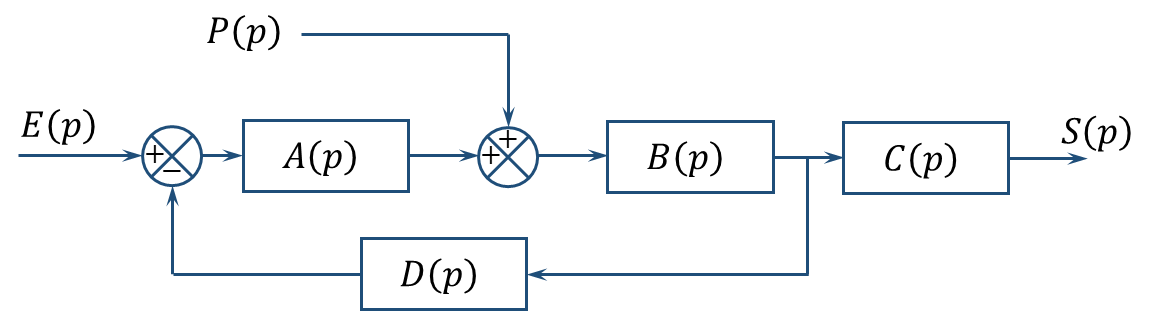
\includegraphics[width=8cm]{fig_02}
\end{center}
	Donner l'écart de trainage pour une rampe de pente $k$. La perturbation sera un échelon d'amplitude $P_0$.
	\begin{reponses}	
	\mauvaise {$\varepsilon_t = \infty$}
	\mauvaise {$\varepsilon_t = \dfrac{k}{1+K}$}
	\mauvaise {$\varepsilon_t = 0$}
	\mauvaise {$\varepsilon_t = \dfrac{1}{1+K}$}
	\mauvaise {$\varepsilon_t = \dfrac{E_0}{1+K} + \dfrac{k}{1+K}$}
	\mauvaise {$\varepsilon_t = \dfrac{1}{K}$}
	\bonne {Je ne sais pas calculer simplement.}
	\end{reponses}
\end{question}\\}

\element{ecart}{
\begin{question}{ecart 15}
Soit le schéma-bloc suivant. On donne $C(p)=K_p \left(1+\dfrac{1}{Tp}\right)$ et $H(p) = \dfrac{K}{p\left(1+\tau p\right)}$.
\begin{center}
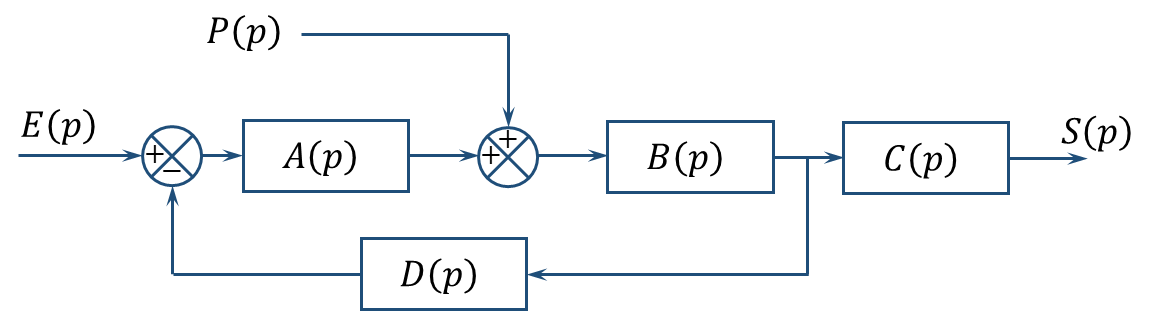
\includegraphics[width=8cm]{fig_02}
\end{center}
	Donner l'écart statique pour un échelon d'amplitude $E_0$. La perturbation sera un échelon d'amplitude $P_0$.
	\begin{reponses}	
	\bonne{$\varepsilon_s = 0$}
	\mauvaise {$\varepsilon_s = \dfrac{E_0}{1+K}$}
            \mauvaise {$\varepsilon_s = \dfrac{E_0}{1+KK_P}$}
	\mauvaise {$\varepsilon_s = \infty$}
	\mauvaise{$\varepsilon_s = \dfrac{1}{1+KK_P/T}$}
	\mauvaise{$\varepsilon_s = \dfrac{E_0}{K}$}
	\mauvaise{$\varepsilon_s = \dfrac{1}{K}$}
	\mauvaise{Je ne sais pas calculer simplement.}
	\end{reponses}
\end{question}\\}



\element{ecart}{
\begin{question}{ecart 16}
Soit le schéma-bloc suivant. On donne $C(p)=K_p \left(1+\dfrac{1}{Tp}\right)$ et $H(p) = \dfrac{K}{p\left(1+\tau p\right)}$.
\begin{center}
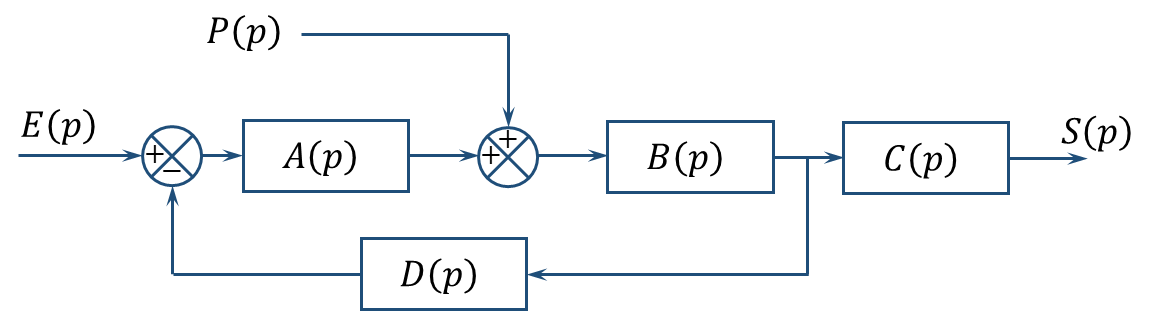
\includegraphics[width=8cm]{fig_02}
\end{center}
	Donner l'écart de trainage pour une rampe de pente $k$. La perturbation sera un échelon d'amplitude $P_0$.
	\begin{reponses}
	\mauvaise {Je ne sais pas calculer simplement.}
	\bonne      {$\varepsilon_t = 0$}
	\mauvaise {$\varepsilon_t = +\infty$}
	\mauvaise {$\varepsilon_t = \dfrac{kT}{K_P K}+\dfrac{P_0T}{K_P K}$}
	\mauvaise {$\varepsilon_t = \dfrac{kT}{K_P K}$}
	\mauvaise {$\varepsilon_t = \dfrac{P_0T}{K_P K}$}
	\end{reponses}
\end{question}\\}






